\documentclass[12pt, a4paper]{book} %Esboco_Tese_Doutorado_2023-09-20
%\documentclass[tese]{abntex2} %Alternativa de tipo de documento (nesse caso, consultar documentação do pacote abntex2)
\usepackage[utf8]{inputenc} %Codificação
\usepackage[brazilian]{babel} %Idioma do documento e ortografia geral
\usepackage{setspace} %Espaçamento de linhas
\usepackage{graphicx} %imagens
\usepackage[hycap]{caption} %legenda
    %\captionsetup[figure]{labelsep=none} %formato legenda
    \usepackage{chngcntr} %fazer contagem global das figuras
        \counterwithout{figure}{chapter} %fazer contagem global das figuras
\usepackage[colorlinks=true, allcolors=blue]{hyperref} %referência cruzada
    \renewcommand{\thefigure}{\arabic{figure}}
\usepackage{xcolor} %cor da fonte
    \definecolor{textcolor}{RGB}{56,74,103} %cor fonte livro Waldheim
    \definecolor{labelcolor}{RGB}{96,86,78} %cor legenda livro Waldheim
\usepackage{tcolorbox} %caixa de texto
%%%%%%%%%%%%%%%%%%%%%%%%%%%%%%%%%%%%%%%%%%%%%%%%%%%%%%%%%%%%%%%%%%%%%%%%%%
\begin{document}

\frontmatter % Seção de pré-texto (capa, sumário, resumo, etc.)

% Title Page
\title{\textbf{Morphoadæquabilitas} 

Um Conjunto de Diretrizes para o 

Projeto de Traçados Urbanos 

Morfologicamente Adequados ao Contexto 

como alternativa ao 

\textit{Modus Faciendi} atual}

\author{Higor Ribeiro da Costa}
\date{Maringá, 2023}

    \maketitle

    \tableofcontents
    \listoffigures %Lista de figuras
    \listoftables %Lista de tabelas

    %\input{resumo} %Arquivo com o resumo da tese

    \mainmatter % Corpo principal da tese

    \onehalfspacing
    

    \part*{}

        \chapter*{Introdução}
        \addcontentsline{toc}{chapter}{Introdução}
        
        Há muito que me pergunto o porquê de nossas cidades serem tão `feias', e penso que isso tenha que ver com seus traçados. Talvez `feio' não seja o melhor termo para descrever esse aspecto da realidade, pois não se trata aqui de um mero juízo estético de minha parte. Porém, \textit{``mentre sul bello si fatica a trovare un parametro congiunto, sul brutto sembra essere meno problematico trovare un terreno comune''} (Daverio, 2022, \textit{s.p.}).
            \footnote[1]{``Enquanto tem-se dificuldade para encontrar um parâmetro conjunto para o [termo] `belo', em relação ao [termo] `feio' parece ser menos problemático encontrar um terreno comum'' (Daverio, 2022, \textit{s.p.}, tradução nossa).} 
        `Se hoje temos tanta tecnologia, por que fazemos casas e prédios, mas, sobretudo, bairros e cidades assim?' Assim `desconjuntados', que `não fazem sentido.' Por que os loteamentos parecem `arranhões de gato' sobre as colinas, com ruas tão íngremes que não permitem a caminhada, dificultam o acesso do transporte, e promovem enxurradas que levam as casas para dentro dos rios? Essa foi uma dúvida que me perseguiu por anos, e, ao começar a entender as causas desse fenômeno, a pesquisa por uma solução – ou pelo menos uma alternativa – pareceu-me imprescindível.

        $<$FIGURA COM LOTEAMENTO DO TIPO `ARRANHÃO DE GATO'$>$

        É necessário salientar que entre o campo da edilícia e o da cidade há uma lacuna considerável. Quero dizer, quando falo em arquitetura `feia,' quero significar aquela arquitetura que não é orgânica – \textit{i.e.,} cujas partes não são interdependentes (veja-se a Villa Capra, de Palladio, em Vicenza) – e que não tem uma relação com seu contexto espaço-temporal. Ou seja, uma arquitetura que não conecta passado e futuro em si própria – em termos de soluções técnicas, organizativas, formais, etc. E explicações para esse fenômeno não nos faltam (Caniggia e Maffei, 2008 [1979]; Strappa, 1995).
            \footnote[2]{Hoje, boa parte de nossa produção arquitetônica é `feia,' por mais `bonita' (esteticamente agradável) que seja – e isso já vem desde, sobretudo, o século XIX. A explicação para isso é dada de maneira muito assertiva por Gianfranco Caniggia e Gian Luigi Maffei (2008 [1979]) e por Giuseppe Strappa (1995). A saber, temos uma `crise' na arquitetura, \textit{i. e.,} vivemos em um momento em que a técnica nos proporciona tantas escolhas possíveis que perdemos o liame com o passado. E, por favor, entendam-me bem. Não estou dizendo que a solução é um retorno romântico ao passado. Não estou dizendo que `a beleza nos salvará'. Mesmo porque, como bem explica Philippe Daverio (2022, \textit{s.p.}), essa frase é uma tradução errônea da obra ``O Idiota'', de Dostoievski, na qual se diz que o mundo seria salvo pela `beleza.' O termo `beleza' aqui, traduzido do russo, não é uma ideia de beleza superficial, de deleite puramente estético, mas diz respeito ao sentido reclamado por Santo Agostinho: a \textit{Pulchritudo Dei, i.e.,} a graça. E esse distanciamento de uma noção de beleza de puro deleite estético vem a calhar na tese que ora escrevo. No entanto, uma olhada para o passado não é de mau tom, sobretudo por duas realidades fundamentais. A primeira é o `\textit{tipo} edilício', \textit{i.e.,} o conjunto de características presentes nas edificações de uma determinada área e que se perpetuam ao longo do tempo. E a segunda é o \textit{`rendimento'}, que é a coerência do \textit{tipo} (Cataldi, 2003, p. 31). Tratei de ambas em minha dissertação (Costa, 2020) e delas devo falar melhor mais adiante.}

        Porém, para as cidades já não temos tantas explicações – talvez, precisamente, pela complexidade do tema. O que é uma cidade `feia'?
            \footnote[3]{No caso das cidades, o que as tornou `feias'? Talvez tenha sido sua dissolução recente? Ou sua expansão pela campanha? Ou a derrubada das muralhas? Mas como pode ter sido a derrubada das muralhas e a expansão das cidades a causa, quando houveram civilizações cujas cidades espalhavam-se por vastas áreas? Mais ainda, como podemos argumentar que isso não é cidade ou é o que `destrói' a cidade quando, enquanto a Europa tinha cidades medievais, o Brasil, segundo Antônio Risério (2013, pp. 18-19), tinha cidades-jardim \textit{avant la letre}? Isso me faz pensar que o problema não reside bem no `o quê', mas sim no `como'. Não é se a cidade tem tal ou qual área, se tem tal ou qual limite, a questão é o como ela se configura: como se configura seu aspecto urbano e edificado. E, já que não vou tratar aqui da edilícia, retrinjo-me apenas ao aspecto urbano, mais especificamente àquele aspecto mais básico e subjacente à cidade: a saber, seu traçado, do qual tratarei adiante, e de suas relações de implantação (no contexto natural) e de sua constituição intrínseca (arranjo).}
        É apenas uma cidade inorgânica? Uma cidade cujo traçado não tem relação com seu contexto – nesse caso, natural e antrópico? E o que fez as cidades se tornarem assim? Ou, em resumo, o que faz com que as novas áreas urbanas tenham, não raro, uma qualidade inferior a antigas áreas urbanas? É certo que vemos as benesses das infraestruturas que não existiam no passado, no entanto, por exemplo, as áreas históricas de cidades antigas fazem os olhos de turistas – tudo bem que atraídos pelo marketing, mas marketing que soube evidenciar as características positivas de tais áreas. E que características seriam essas? Posso apontar duas, pelo menos. A primeira é a coerência entre as edificações da área, não raro em um \textit{continuum} de fachadas que cria um grande cenário urbano – cenário autêntico. E a segunda é o formato do traçado que lhes dá suporte, com todos os seus elementos – e isso é o que me interessa.

        \begin{center}
        . . . . .
        \end{center}

        No fim de minha dissertação, cheguei à conclusão de que é possível projetar traçados urbanos morfologicamente adequados ao contexto. E explico o que quero dizer com isso. `Contexto' aqui é o conjunto de estruturas naturais e antrópicas de uma área com suas respectivas características, suas variáveis. `Morfologicamente adequado' quer dizer aquilo que já é, desde sua concepção, coerente com o formato das estruturas do contexto dado pela realidade. E traçado urbano é a marca das estruturas urbanas que o homem desenvolve.

        No caso das estruturas naturais, o que tomo por mais importante é a orografia, a terra com a sua forma, que é sobre onde se assentam as estruturas que o homem desenvolve, seguida pela hidrografia. Uma área pode ser mais íngreme ou suave, mais ou menos extensa, e seu relevo possui uma hierarquia latente, que pode ser destrinchada por meio de cumeadas, pontos de distribuição, assim como por talvegues e pontos de encontro. E, no caso das estruturas antrópicas, temos parcelamentos rurais precedentes, franjas urbanas com loteamentos, e diretrizes viárias. Com isso, temos ruas e avenidas, lotes urbanos e glebas rurais com seus limites. Cada uma dessas estruturas naturais e antrópicas desenvolve uma relação de interdependência, existencial – pois algumas não podem existir sem outras – e morfológica, por meio de seus formatos poligonais e consequentes angulações – bidimensional ou tridimensionalmente. 

        Ou seja, quando digo que um traçado urbano deve ser `morfologicamente adequado ao contexto', quero implicar que cada um de seus elementos (sobretudo ruas, praças, demais espaços abertos, e os lotes e quarteirões que derivam de sua disposição) deve, na máxima medida possível, seguir, primeiro, os formatos dados pela estruturação natural, e segundo, os formatos dados pelos elementos da estruturação antrópica. E isso se opõe ao \textit{laissez-faire} dos traçados `hilemórficos' concebidos \textit{a priori} e só depois `adaptados' à realidade, que se impõe forçosamente ao projetista contrariado. Um traçado `adequado' é diferente de um traçado `adaptado'. É a morfogênese planejada contraposta ao hilemorfismo autômato. 
            \footnote[4]{\textit{``The hylomorphic model has dominated the relationship between matter and form within Western culture. The term ‘hylomorph’ indicates what is needed to design, for example, a table. It derives from \textnormal{hyle}, meaning wood, and morph, meaning form. So when we design a table by means of the hylomorphic model, we take a form \textnormal{(morph)} – the image of the table we would like to design – and press it into the wood \textnormal{(hyle)} – the material by which the image should come alive. The effect is a copy, a representation of what we imagined a table should look like."} (Trummer, 2009).}

        \begin{center}
        . . . . .
        \end{center}

        Durante aquela pesquisa, da qual a presente tese não é senão a continuação, desenvolvi o conceito de `\textit{rendimento} urbano' – que afirma que deve existir uma ``coerência intrínseca entre o traçado da forma urbana e o contexto natural" (Costa e Rego, 2019, p. 7); e projetei um traçado urbano hipotético sobre uma área urbana consolidada, comparando-o com o traçado existente e com a legislação local em vigor. Com isso, verifiquei ser possível projetar traçados urbanos `de qualidade' (Costa, 2020, p. 106). Traçados com bom \textit{rendimento} urbano.

        O que fiz na dissertação foi uma simulação baseada na síntese de um novo conceito (o \textit{rendimento} urbano) e em um estudo de caso (a partir do qual foram extraídos parâmetros para a avaliação desse conceito). Eu queria mostrar que um traçado urbano adequado ao sítio tinha lugar no mundo contemporâneo das cidades planejadas \textit{a priori}, posto que, hoje, um processo de desenvolvimento gradual da estrutura urbana, do traçado urbano, parece já não ter lugar – pois o \textit{status quo}, hoje, é o da morfogênese substituída pelo hilemorfismo. 

        Outrora, as ruas não eram senão a afirmação de percursos pré-existentes, sulcados ao longo do tempo no relevo do território por inúmeras gerações que nos precederam – segundo Caniggia e Maffei (2008), remontando ao período neolítico. Esses percursos, primitivamente utilizados apenas como rotas de passagem, passaram a ser a estrutura de acesso a áreas inicialmente de caça e coleta, posteriormente de cultivo, até chegar à sua partição em propriedades. E, nos locais mais propícios, tais percursos tiveram seus formatos consolidados, consagrados na matéria, por meio das fachadas as edificações que os margeavam. Era a formação do que, no universo lusófono, chamamos de ``rua", com a série de edificações a ela rentes.

        Observando esse processo, não é difícil perceber que eram os saberes tradicionais da consciência espontânea e a acomodação ao legado das gerações anteriores que capitaneavam a formação de ruas – ou melhor, de `percursos edilícios'. E o direito consuetudinário os mantinha com suas características. Hoje, porém, temos leis positivistas que ditam de antemão como um projeto pode ser feito – seja um arruamento, um parcelamento ou um \textit{masterplan}. E é esse projeto que vai moldar a realidade material que constituir-se-á em um sítio. É toda uma outra dinâmica. Assim, naquele momento decidi projetar um novo traçado urbano adequado às exigências da contemporaneidade, porém projetado a partir de um esquema `à antiga'.

        Para projetar esse novo traçado urbano 'à antiga',
            \footnote[5]{Parece contraditório falar em morfogênese – em um processo totalmente espontâneo – e, no entanto, projetar um traçado – ou seja, executar uma atividade apriorística, ainda que esta leve em conta o processo de formação de traçados de morfogênese espontânea. No entanto, o paradgima atual exige o projeto. E, portanto, não posso me eximir dessa realidade e simplesmente deixar a cargo da iniciativa individual a execução de novos traçados urbanos – ainda mais em um momento no qual a consciência espontânea e o imaginário coletivo encontram-se em uma espécie de caos (Caniggia e Maffei, 2008; Carvalho, 2012), dada a miríade de possibilidades de se fazer algo. Mais ainda: dentro da nossa realidade atual existem inúmeros projetistas, gestores, pesquisadores, docentes e alunos que projetam traçados urbanos, e que não vão ceder aos caprichos de um desconhecido.} 
        lancei mão de um estudo de caso, fazendo uma leitura morfológica do traçado original projetado para a cidade de Maringá-PR, reputado como uma solução moderna e adequada às pré-existências do sítio – concomitantemente com o parcelamento rural da Companhia (CTNP/CMNP)
            \footnote[6]{A Companhia que desenvolveu o território rural no qual foi `plantada' a cidade de Maringá era subsidiária da \textit{Paraná Plantantions Ltd.}, de capital britânico, tendo o nome de `Companhia de Terras Norte do Paraná.' No entanto, no ínterim da Segunda Guerra Mundial, com a retração do capital britânico investido no exterior para realocação nos esforços bélicos, por ordem da Coroa, e a aquisição da Companhia por investidores brasileiros, a mesma passou a se chamar `Companhia Melhoramentos Norte do Paraná,' momento no qual Maringá foi pensada e seu traçado encomendado (Rego, 2009).} 
        que encomendou o projeto (Rego, 2009, 2001; Rego \textit{et al.}, 2004; Bonfato, 2008; Beloto, 2015; Meneguetti, 2007; Kohlhepp, 2015; Waibel, 1949). A partir disso, extraí parâmetros de avaliação do \textit{rendimento} urbano para novos traçados urbanos. E, para provar que os era possível utilizar, projetei esse novo traçado urbano sobre uma área da atual cidade de Maringá – outrora parte da área rural parcelada pela Companhia, fora dos limites do plano original da cidade, e com uma `qualidade' inferior a este. Feito isso, desenvolvi um comparativo quantitativo entre os dois traçados urbanos, comparando-os um com o outro, e com a legislação atual (\autoref{fig:comparativo_tracados}), verificando ser possível projetar um novo traçado urbano adequado ao sítio com uma `qualidade' superior ao \textit{modus faciendi} atual e mantendo índices semelhantes, desde que aplicando o conceito de \textit{rendimento}.

        \begin{figure}[h]
            \centering
            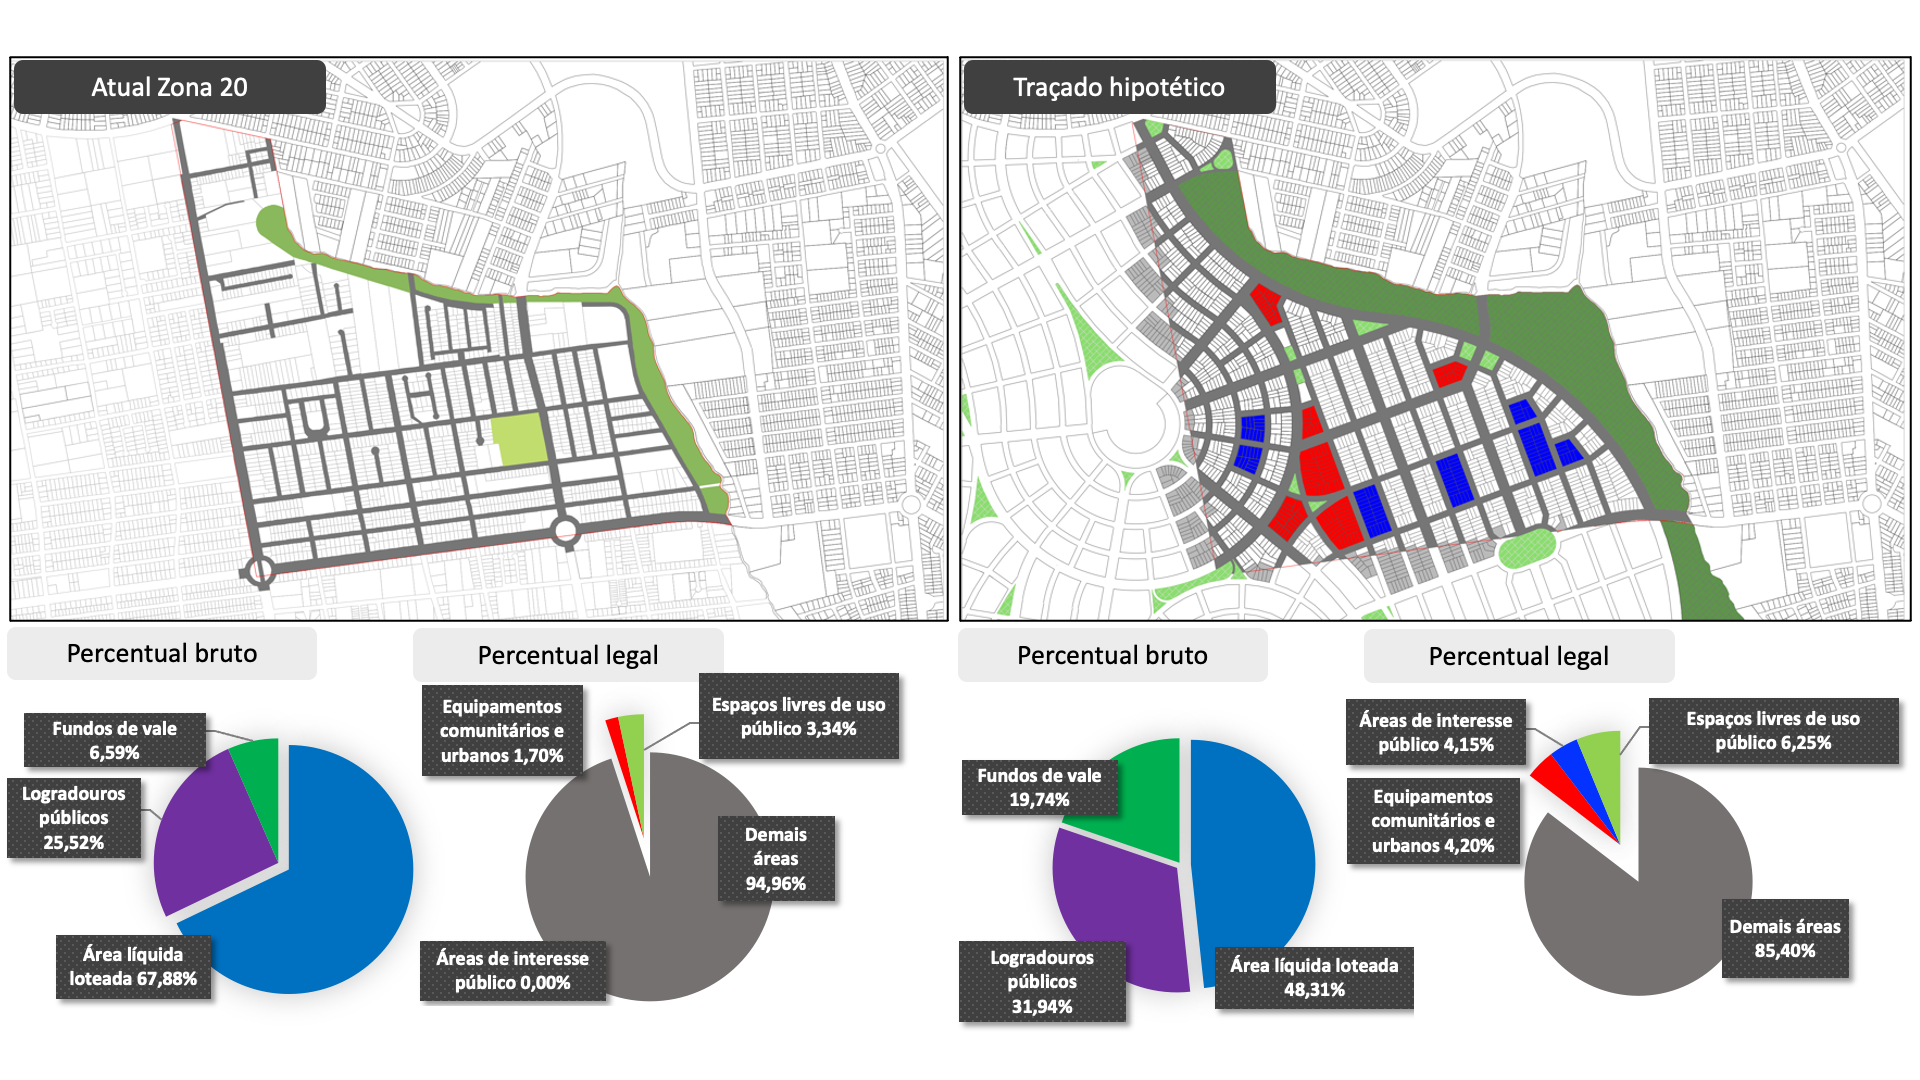
\includegraphics[width=1\textwidth]{/Users/Pancratii/GitHub/phd/Sections/Projeto_de_Pesquisa_2023-03-18_Teste/Pictures/comparativo_tracados.png}
            \captionsetup{labelfont=bf}
            \caption{Comparativo entre o traçado existente (à esquerda) e o traçado hipotético projetado (à direita). \textbf{Fonte:} Costa, 2020 (adaptado).}
            \label{fig:comparativo_tracados}
        \end{figure} 

        \begin{center}
        . . . . .
        \end{center}

        A principal evidência que me trouxe até aqui foi a existência de traçados urbanos adequados à topografia do sítio e de traçados feitos à revelia do relevo – estes últimos relacionados a diversos problemas, sendo oriundos daquilo que chamo '\textit{modus faciendi} atual' (Costa \textit{et al.,} 2020). Pude perceber isso em diversas cidades, e não foi diferente com Maringá-PR, meu local de estudo e experimentação até o momento. Nela, o traçado do plano original da cidade – projetado por Jorge de Macedo Vieira – se encaixa na primeira categoria, e o traçado das expansões urbanas – desenvolvido sobre o parcelamento rural da Companhia – na última.  

        O primeiro grupo congrega traçados urbanos orgânicos, com elementos interdependentes, não serializáveis ou intercambiáveis. Tais traçados podem ser oriundos tanto de um desenvolvimento espontâneo como de um processo de planejamento. E, em ambos os casos, o que se vê é um processo de formação ou desenvolvimento projetual mais complexo e elaborado, e, consequentemente, mais prolongado no tempo, adequando-se de modo particular às características físicas do sítio. 

        Já o segundo grupo congrega traçados não-orgânicos e intercambiáveis, oriundos do \textit{modus faciendi} atual. Neles, é possível observar uma lógica hilemórfica subjacente, na qual prioriza-se um retorno financeiro ligado à venda de lotes, dispostos ora em quadras ortogonais (loteamentos comuns), ora em quadras formadas por ruas curvas que levam `do nada a lugar nenhum' (loteamentos de `alto padrão').
            \footnote[7]{O \textit{grid} de quadras e lotes ortogonais apresenta, assim como nos acampamentos militares do passado (Kostof, 2014), um desenho abstrato – a grelha – que só \textit{a posteriori} é confrontado com o relevo e deformado pela topografia – na forma de grandes e íngremes ladeiras, por exemplo. Ou seja, o que conta no \textit{modus faciendi} atual é a `economia': de tempo, de dinheiro e de neurônios – talvez até de boa vontade, a depender do caso. No caso do \textit{grid} dos loteamentos comuns, conta a rapidez da venda e obtenção dos lucros. E no caso dos loteamentos fechados, vendidos como `jardins', por exemplo, conta o marketing como agregador de valor a um traçado urbano que não necessariamente é orgânico.}

        O resultado da aplicação indiscriminada de traçados abstratos, de concepção alheia ao contexto no \textit{modus faciendi} atual são ``territórios descontínuos e paisagens contraditórias'' (Strappa, 2018, p. 11, tradução nossa). Loteamentos e loteamentos que `brotam' como fungos a partir das cidades, de suas franjas e conexões.
            \footnote[8]{A expressão `fungos' foi utilizada pelo professor Philippe Daverio (2018), no contexto das cidades italianas, cuja expansão se dá de modo diferente ao que ocorre no Brasil (cf. Indovina, 2009). No entanto, tanto lá como em ultramar, muitas vezes ocorre o surgimento de empreendimentos urbanos (\textit{i.e.,} loteamentos) em locais inusitados, conectados às áreas urbanas consolidadas apenas por meio de uma pequena estrada, assim como os fungos também se reproduzem e espalham `em rede'. Portanto, a analogia permanece válida.} 
        Geram-se, assim, manchas urbanas formadas por traçados desconexos entre si. E o que se percebe é uma tendência à segregação dessas novas áreas urbanas, bem como uma diminuição da mobilidade, com a sobrecarga das poucas vias de acesso – em geral íngremes.

        Além disso, não há uma distinção clara ou uma integração sustentável entre a mancha urbana e o território natural e produtivo. Diversas ruas fazem `incursões' em áreas que, por sua morfologia e características naturais, deveriam ser preservadas. E, desse modo, o que ocorre não é uma integração entre a cidade e o campo, ou o dissolver das estruturas urbanas no território circunstante, mas sim uma espécie de `corrupção' de todos: cidade, campo e natureza.

        \begin{center}
        . . . . . 
        \end{center}

        É verdade que, sobretudo na primeira metade do século XX, houveram ideários a tentar sanar essa situação, focando sobretudo na cidade enquanto habitat humano que deveria ser melhorado: estética, logística e funcionalmente. E isso por meio da relação da cidade-campo, da densidade, de determinados arranjos formais do traçado ou da dissolução da cidade tradicional em favor de utopias. Enquanto isso, nos últimos 50 anos, viu-se um emergir de considerações ambientais, não mais da cidade, mas da `paisagem'.
            \footnote[9]{As definições de `paisagem', \textit{`landscape'} e \textit{`paesaggio'} serão destrinchadas no momento oportuno.} 
        E, mais recentemente, podemos ver a ideia de \textit{`landscape'} enquanto \textit{`framework'} das cidades e regiões dentro do chamado \textit{`landscape urbanism'} (Waldheim, 2016). No entanto, em nenhum desses casos é possível identificar um estudo metódico do processo de morfogênese, sobretudo dos assentamentos espontâneos. Isso só se fez visível no arcabouço teórico-metodológico da escola italiana de tipomorfologia urbana – pouco conhecida e divulgada, precisamente por ser uma 'escola' e não um 'ideário' com princípios a aplicar por toda parte. E, ainda assim, a escola italiana trata de leitura e análise urbano-territorial, no entanto sua ênfase projetual se dá na escala das edificações, ou em projetos urbanos (\textit{`masterplan'}). Ou seja, ou oito, ou oitenta.

        Desse modo, não existem diretrizes claras para projetar traçados de maneira coerente e orgânica, sobretudo conforme o conceito de \textit{rendimento} urbano. Ademais, mesmo nos casos dos quais é possível extrair alguma diretriz, percebe-se, como sobredito, que tais casos não são feitos do mesmo modo que os traçados urbanos costumeiramente são feitos – ao menos no Brasil –, \textit{i. e.,} por loteamentos (bidimensionais) – e não à maneira de \textit{masterplan}, em que os edifícios (tridimensionais) – ou ao menos seus volumes – são projetados \textit{a priori} (Maretto, 2018; Maretto, Costa e Rego, 2023); afinal, estou falando de `traçado' (\textit{urban shape}) e não de `forma' (\textit{urban form}). E é diante desse problema que me pergunto: `como projetar um traçado urbano morfologicamente adequado ao contexto?' 

        O que pretendo, portanto, é desenvolver um conjunto de diretrizes para o projeto de traçados urbanos. Traçados esses que devem ser morfologicamente adequados. Diretrizes essas que possam ser aplicadas em diferentes contextos. E meu intuito com isso é gerar uma alternativa ao \textit{modus faciendi} atual. Para isso, eu preciso ampliar o horizonte do conceito de \textit{rendimento} para além do traçado urbano enquanto algo estanque, tornando-o aplicável na dinâmica da realidade. Ou seja, devo relacionar o conceito de \textit{rendimento} urbano com o processo de expansão urbana e com as estruturas naturais e antrópicas que lhe servem de \textit{framework} – nesse caso, expansões extra-urbanas, peri-urbanas e/ou intra-urbanas.
            \footnote[10]{Eu falaria aqui, também, de reestruturação urbana – no sentido caniggiano do termo. No entanto, penso que estabelecer um modo de fazer cidades e territórios adequado ao contexto servirá tanto para `expansões' quanto para `reestruturações' urbanas.} 
        E, a partir disso, desenvolver um artefato (conjunto de diretrizes) que possa ser utilizado por todos aqueles que projetam traçados, e, com isso, produzem cidades e territórios: profissionais, pesquisadores, docentes, alunos. Destarte, se falar em mudança de paradigma é de uma presunção deveras arrogante, faz-se mister, porém, falar em `alternativa' ao modo de fazer traçados urbanos hoje em voga.

        \begin{center}
        . . . . .
        \end{center}

        Uma justificativa razoável para a presente empresa é a ausência de estudos prescritivos para traçados urbanos sob a luz do \textit{rendimento} urbano e de sua prerrogativa de coerência entre traçado e contexto. No campo da morfologia urbana, existem estudos de observação e análise de traçados urbanos, como a metodologia \textit{Morpho} (Oliveira e Silva, 2013; Oliveira e Medeiros, 2016), mas que não consideram a topografia; ou estudos que consideram as formas do terreno no território e outros fatores ligados à sustentabilidade ambiental (Fanta \textit{et al.,} 2022), mas que não adentram no tocante específico dos traçados urbanos e de seus formatos. Ambos de caráter não-prescritivo. Neles, vê-se a ausência de diretrizes prescritivas para o desenho das cidades, sobretudo diretrizes que agreguem \textit{savoir-faire} de diferentes áreas do conhecimento. Há diretrizes, e até métodos para a análise que dá suporte a um possível processo de projeto, mas não uma prescrição endereçada diretamente a tal. Há ainda o método de projeto desenvolvido no âmbito dos workshops W.A.M. (Maretto, 2018), e aquele presente no trabalho de Saverio Muratori para o programa habitacional INA-Casa (Maretto, Costa e Rego, 2023) – ambos prescritivos. Porém, em ambos, ainda que havendo alguma consideração pela topografia (sobretudo no exemplo muratoriano), parte-se de uma realidade edificada pré-existente, com tecidos urbanos históricos, ou em áreas novas (ou de intervenção) nas bordas de uma realidade construída já consolidada. E isso sem falar que aqui tratamos de projetos \textit{à la masterplan}, ou seja, de um processo que depende do arquiteto e de um ente que possa levar a cabo toda a empreitada, diferente do processo de formação da cidade, com seus diferentes atores e fontes de receita (Alexander \textit{et al.,} 2013).

        Ou seja, não há diretrizes atuais para o projeto de traçados urbanos partindo da característica mais crua e rudimentar de uma cidade, daquilo que lhe é subjacente, a saber: a forma de sua estruturação natural. Esta, com toda sua complexidade, reflexo de relações orgânicas de interdependência entre orografia e hidrografia – moldadas pelo clima, regime pluviométrico, e tipos de solo – recebe todos os impactos do processo de urbanização. Mais um fator a ser observado em um conjunto de diretrizes – o da sustentabilidade ambiental, vinculada ao formato dos traçados, com a qualidade inerente à sua morfologia. Adaptação dos formatos do traçado urbano, que são subjacentes às formas edificadas e que conferem qualidade ao ambiente construído, disposto sobre um relevo natural. Estes são os pontos fulcrais que justificam um estudo como a tese aqui proposta, pois, por meio de um conjunto prescritivo de diretrizes que visa incrementar um processo já existente de projetação de traçados urbanos, explicita-se ser possível associar \textit{rendimento} urbano e ‘rendimento’ econômico, mostrando que os diversos interesses dos diferentes atores que atuam na cidade podem convergir para um bem comum, no qual todos saiam ganhando.

        Ademais, se é verdade que consegui projetar um traçado urbano adequado a um determinado contexto, não necessariamente é verdade que uma outra pessoa o conseguirá fazer em outro contexto. Faz-se mister pôr à prova o estratagema que utilizei. E como tornar isso palpável? Por meio de um software ou algoritmo, no qual fosse necessario fornecer apenas algumas instruções, dar um \textit{input}? Bom, nesse caso eu precisaria de uma equipe, e diretrizes já delineadas e organizadas metodicamente, coisa que é inviável no prazo de quatro anos de um doutorado – ao menos para um leigo em linguagem de programação. Então por meio de um método, com um passo-a-passo? Não necessariamente, posto que isso engessaria a aplicação do projeto quando em diferentes contextos e circunstâncias. Bem, nesse caso, por exclusão, cheguei à determinação de que são necessárias diretrizes de projeto, um conjunto de diretrizes para o processo de projetar traçados urbanos morfologicamente adequados ao contexto. 

        \begin{center}
        . . . . .
        \end{center}

        %Método
        Para desenvolver tais diretrizes, lanço mão da \textit{Design Science Research} (DSR) como método de pesquisa (Dresch \textit{et al.,} 2013; Lacerda \textit{et al.,} 2015), por ser um método prescritivo que visa a melhoria de processos já existentes. No caso em questão, prescritivas são as diretrizes de projeto e a realidade ou processo existente a ser melhorado é o processo de projeto de traçados urbanos.

        Fulcrais na DSR são: o desenvolvimento de um `artefato' (aqui, o conjunto de diretrizes), e a avaliação e comunicação dos resultados por e para os \textit{stakeholders} (que, no caso em questão, são profissionais, gestores, pesquisadores, docentes e estudantes que lidam com o processo de projeto de traçados urbanos). Tal método de pesquisa é constituído por fases, sendo elas: (1) consciência do problema; (2) sugestão; (3) desenvolvimento; (4) avaliação; e (5) conclusão. Tais fases se retroalimentam entre si, e seus produtos são: (a) proposta; (b) esboço; (c) artefato; (d) mensuração; e (e) resultados.

        Na presente pesquisa, associo a DSR com estratégias como estudo de caso, modelagem, simulação e grupos focais, de modo a compreender a realidade na qual pretendo intervir, identificar diferentes possibilidades dentro da realidade em questão, desenvolver um arcabouço de soluções, e verificar se tais soluções são aplicáveis em outras realidades.

        Assim, para preencher tal lacuna e alcançar o objetivo acima proposto, na senda da \textit{Design Science Research}, fazem-se necessárias as seguintes etapas, que se refletem no delineamento da pesquisa: 
            \begin{itemize}
                \item revisar conceitos e métodos; 
                \item efetuar um estudo de caso sobre Maringá, com levantamento documental e cartográfico, leitura morfológica e revisão de literatura acerca do projeto original, das expansões urbanas, do parcelamento rural e das diretrizes viárias, bem como revisão da legislação atual e entrevistas com \textit{stakeholders} para entender as premissas, motivações e o processo de projeto no \textit{modus faciendi} atual; 
                \item buscar soluções semelhantes que já tenham sido aplicadas (como \textit{guidelines, patterns,} métodos, leis, manuais, livros) na classe de problema em questão (\textit{i.e.,} ausência de método de projeto), além de selecionar e esboçar um tipo de solução a ser desenvolvida;
                \item estabelecer um protocolo para o desenvolvimento do conjunto de diretrizes; 
                \item desenvolver um conjunto de diretrizes piloto por meio de modelagem e simulação (com traçados urbanos hipotéticos); 
                \item avaliar um conjunto de diretrizes por meio de comparativo com legislação, situação, morfologia e \textit{modus faciendi} atuais (para aferir viabilidade), e por meio de grupos focais (para avaliar aplicabilidade em outros contextos); e, por fim, 
                \item refinar e sintetizar as diretrizes do conjunto.
            \end{itemize}

        \begin{center}
        . . . . .
        \end{center}

            \section{Estrutura da Tese}

            A presente tese, destarte, é estruturada em três 'partes': a primeira, 'consciência'; a segunda, 'desenvolvimento'; e a terceira, 'avaliação'. Na primeira parte, estão presentes o estado da arte, a análise do contexto em que a tese será aplicada – qual circunstância será melhorada/refinada – e a definição de novos termos e conceitos pertinentes à tese aqui desenvolvida. Na segunda, as diretrizes de projeto são extraídas de projetos piloto de traçados urbanos seguindo um protocolo. E, por sua vez, a terceira parte é uma avaliação das diretrizes de projeto por parte dos \textit{stakeholders} do processo de projeto de traçados urbanos, \textit{i.e.,} profissionais, gestores, docentes e estudantes – ou seja, nessa última parte as diretrizes são testadas por terceiros alheios à feitura desta tese, de modo a avaliar se tais diretrizes (artefato) são realmente aplicáveis à realidade, ao meio para o qual foram desenvolvidas, a saber, escritórios (públicos ou privados), ateliês de projeto e salas de aula; e, em seguida, são sistematizadas.

            A primeira parte é dividida nos seguintes capítulos:
            \begin{itemize}
                \item O traçado da cidade: no primeiro capítulo é feita a revisão assistemática de literatura
                
                \item Maringá, um novo estudo de caso: no segundo capítulo é feito um estudo de caso sobre Maringá, com levantamento documental e cartográfico, leitura morfológica e revisão de literatura acerca do projeto original, das expansões urbanas, do parcelamento rural e das diretrizes viárias, bem como revisão da legislação atual.
                \item A escolha de uma solução: revisão sistemática de literatura para identificar 
            \end{itemize}

            Na segunda parte, encontra-se o capítulo intitulado `o projeto de traçados hipotéticos'
                Parâmetros: quantitativos (número de lotes, área verde por habitante, área loteável, área pública), leis, etc.
                O projeto de traçados hipotéticos: aqui, apresento três pilotos, projetos hipotéticos de traçados urbanos. O primeiro foi desenvolvido durante o mestrado, sozinho, sobre um promontório inteiro, ou seja, uma espécie de \textit{tabula rasa} e um piloto inicial de traçado urbano. O segundo traçado foi desenvolvido durante enquanto orientei um projeto de iniciação científica, considerando algumas pré-existências antrópicas da área estudada, como diretrizes viárias, avenidas e faixas de domínio pré-existentes; portanto, um piloto de desenvolvimento semi-autônomo das diretrizes por parte de \textit{stakeholders} (eu e o aluno orientado), ao mesmo tempo que abarcando áreas intra-urbanas, o que indica a possibilidade de uso das diretrizes em áreas urbanas sub-utilizadas, ou na pesquisa e no estudo comparativo (acadêmico) de possíveis alternativas ao modo como atualmente se projetam traçados urbanos. E o terceiro foi desenvolvido no âmbito desta tese, considerando um processo de expansão urbana cujos módulos são os lotes rurais paulatinamente ocupados por loteamentos estruturados por uma estrutura comum (eventualmente um \textit{framework}). Neste capítulo, assim, são apresentados tais traçados e o passo-a-passo de seu desenvolvimento projetual, o que nos leva ao capítulo seguinte.
                Diretrizes projetuais: Neste capítulo, as diretrizes projetuais extraídas do desenvolvimento projetual dos pilotos são sistematizadas dentro de um esquema que permite diferentes alternativas, de modo a proporcionar diversas soluções projetuais em diferentes contextos, porém, sempre mantendo a mesma qualidade de morfoadequação do traçado ao contexto.
                Comparativo com existente: (número de lotes, área verde por habitante, área loteável, área pública), leis, etc.
                
            Já na terceira parte, encontram-se os seguintes capítulos:
            \begin{itemize}
                \item Grupos focais e \textit{feedback}
                \item Diretrizes projetuais
            \end{itemize}


    
    \part[Consciência]{Consciência}

        \chapter[O traçado da cidade]{Revisão de literatura}

            Alguns parágrafos atrás apontei duas características subjacentes às cidades admiradas por sua `beleza', a saber: o formato (ou configuração) do traçado – do qual falarei adiante – e o \textit{continuum} de fachadas, que deriva de duas realidades latentes na edilícia e estão condensadas nos conceitos de \emph{`tipo'} e \emph{`rendimento'}. E me permito aqui fazer uma analogia com o mundo dos automóveis, ironicamente, para ilustrar essas realidades.

            Se observarmos todos os carros produzidos até hoje (salvo exceções que salpicam de tempos em tempos), todos têm: quatro rodas, um motor, um habitáculo. Certo? E isso está associado com a `função' do automóvel, a saber, ser um veículo que leva passageiros de um ponto a outro. E isso o carro tem em comum com seu ancestral, a carroça, e até com a liteira. Por ter quatro rodas, o carro necessita de pára-lamas, por exemplo. Por ter um motor a combustão (por enquanto), o carro precisa de uma abertura para entrada de ar. Por ter um habitáculo, o carro precisa de portas. E para ser guiado, ele precisa de um volante. E para que seu motorista tenha uma boa utilização dele, ele tem um cockpit e uma série de equipamentos. E tudo isso reverbera na \textit{forma}, no \textit{design} do automóvel. Correto? 

            Muito bem, todas essas são características tipológicas de um automóvel relacionadas à sua `função' e à sua `forma', que segue sua função. E quanto mais um carro é diferente dos outros em suas `linhas', menor será o seu \textit{rendimento} em relação ao conjunto, \textit{i.e.,} ao mundo automotivo. E o que ocorre é que, das duas uma: se ele cai no gosto do freguês, ele `puxa' o mundo automotivo em uma nova direção; ou, se isso não acontece, ele cai no esquecimento. Basta compararmos um Citroën DS 1955 com um Reliant Regal 1953, dois carros com baixo \textit{`rendimento'} – no sentido mencionado – e com dois destinos completamente diferentes. Assim, o \textit{tipo} se forma como um patrimônio de soluções que deram certo, por assim dizer, enquanto que o \textit{rendimento} é a submissão de algo novo a esse patrimônio já existente.
	
	        \begin{center}
		    . . . . .
	        \end{center}

            No mundo das edificações ocorre algo semelhante – ou deveria acontecer. Tomemos as casas como exemplo. As casas acumulam características relacionadas à sua função de residência, de moradia, e, mais primitivamente, de recinto, de abrigo do mundo exterior – e isso se vê bem quando observamos nossa arquitetura do dito período colonial. E isso tanto em planta quanto em fachada. Tudo isso era passado ao longo das gerações e apenas a linguagem mudava de tempos em tempos (aquilo que alguns chamam de `estilo'). Pois bem, isso mudou nas últimas décadas com o avanço da técnica. A cada novidade, buscamos novas formas. Com isso perdemos nosso liame com o passado. E o mesmo ocorre com os traçados urbanos. E, dito isso, voltemos à nossa hipotética pergunta inicial: `por que construímos cidades feias, ou melhor, desarmônicas?' 

            Pensando bem, talvez valha pensar em `o que faz uma cidade ser desarmônica' antes de perguntar o `porquê' disso. E, afinal, qual a razão de saber o `porquê' de uma cidade ser desarmônica? É apenas para trazer à luz o problema? Não penso, pois, embora uma tese científica usualmente se ocupe de identificar e estudar fenômenos, eu sou arquiteto, e, como tal, pretendo desenvolver algo propositivo. E, para isso – aí sim – preciso entender (racionalmente) o fenômeno que fere meus olhos (sentidos), a saber, a tal `feiúra' ou `desarmonia' das cidades. 
	
	        Em princípio, o que salta aos olhos é um aspecto estético, de olhar e ver que as coisas `não encaixam', que não formam um conjunto harmonioso entre si. O cineasta italiano Pierpaolo Pasolini (1974) já dizia que a forma da cidade só se manifesta, aparece e se revela quando confrontada com um cenário natural. E que, portanto, o problema das cidades e o problema da conservação da natureza que as rodeia são uma coisa só.
                \footnote[4]{“La forma della città si manifesta, appare, si rivela se confrontata con un fondale naturale. Proprio la forma della città di Orte pare in quanto tale perché sulla cima di questo colle bruno divorato dall’autunno, con questa brunatura davanti, e contro il cielo grigio. Ora, quelle case che ti ho citato prima (...) vengono turbare soprattutto il rapporto della forma della città e la natura. Ora, il problema della città e il problema della salvezza della natura che circonda la città sono un problema unico. Ma sempre si pone il problema di rispettare il confine naturale tra la forma della città e la natura circostante.” PASOLINI, 1974.} 
            Confesso sou tentado a sonhar com um mundo em que as cidades medievais não deixaram sua forma de polos compactos em meio à campanha, em um território bem estruturado ao longo do tempo. Porém, é necessário lidar com a realidade – pois minha ideia romântica ignora todos os problemas do passado e pinta aquele mundo de rosa.  Nesse sentido, é preciso ver o que está subjacente ao que Pasolini percebeu. O que é que está por trás das mudanças ocorridas nas cidades? 

            Em parte, é possível identificar o que houve, se pensarmos que a edilícia mudou: o abandono, ou melhor, o esquecimento do \textit{tipo} ajuda a entender muita coisa, posto que esse é o primeiro aspecto que salta aos olhos quando estamos `dentro' da cidade, inseridos nela. Porém, esse é apenas um aspecto.\footnote[5]{E, em parte, esse é um aspecto `apenas' visual – apenas em parte, pois a noção de \textit{tipo} perpassa da edificação ao território (CANIGGIA E MAFFEI, 2008). } Há ainda um outro aspecto, que é estrutural. E que está relacionado ao traçado urbano. Assim, se podemos deduzir uma solução em relação às edificações – ou ao menos um vislumbre do que fazer (DALLA NEGRA, 2015; IEVA, 2015; SCARDIGNO, 2021), como nos projetos de Saverio Muratori (MARETTO, COSTA E REGO, 2023) –, o mesmo não se dá em relação ao traçado urbano. E aqui faz-se necessário elucidar a diferença entre duas dimensões a que devemos atentar ao analisar essa as cidades. 
	
	        A primeira é a sua '\textit{forma},' aquilo que podemos enxergar diretamente com os olhos e apalpar com mais facilidade na cidade – isto porque a \textit{forma} urbana (\textit{the urban form}) é, por definição, tridimensional, eu diria até `mais material'. A segunda dimensão é o `traçado urbano' (\textit{the urban shape}), o `formato' da \textit{forma,} o contorno que a delineia, o que, por definição, é bidimensional, e, por isso mesmo, `menos material', ou seja, perceptível pelos sentidos apenas de maneira latente e apenas observável por meio de um processo de abstração que envolve a apreensão da \textit{forma} e sua posterior representação. Representação essa mais esquemática e abstrata do que o seria uma representação direta da \textit{forma} – basta pensar na diferença entre uma pintura, como as de Caspar van Wittel (\autoref{fig:popolo}), e um mapa, como o de Giambattista Nolli (\autoref{fig:nolli_popolo}).

            \begin{figure}[h]
	            \centering
	            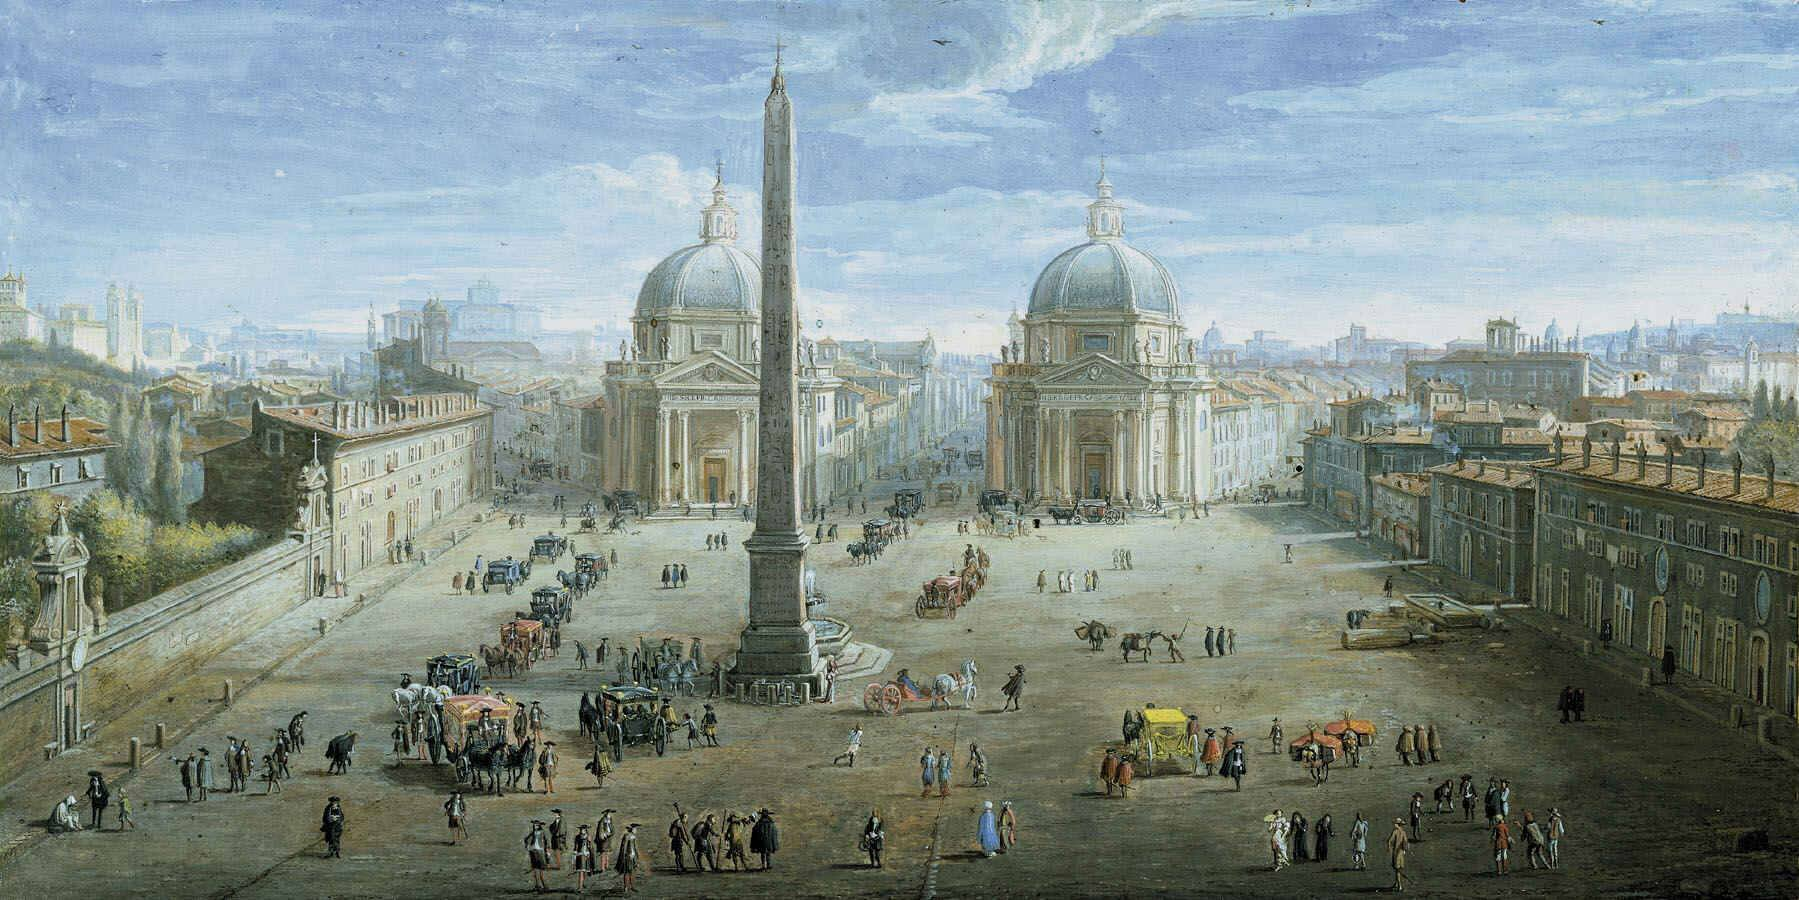
\includegraphics[width=1\textwidth]{/Users/Pancratii/GitHub/phd/Sections/Projeto_de_Pesquisa_2023-03-18_Teste/Pictures/popolo.jpeg} 
	            \captionsetup{labelfont=bf}
	            \caption{Vista da \textit{Piazza del Popolo}, em Roma, por Caspar Van Wittel (1652–1736). \textbf{Fonte:} Wikimedia Commons / Sotherby's (coleção privada).}
	            \label{fig:popolo}
            \end{figure}   

            Discorramos rapidamente sobre a ideia de \textit{forma} e traçado. Traçado é o particípio do verbo traçar, \textit{i.e.,} desenhar traços, riscar, sendo o ato ou efeito desse mesmo verbo, resultando, portando, em um `conjunto de traços', ou, no nosso caso, no `desenho que representa uma estrutura arquitetônica ou urbanística', o que é equivalente a dizer `planta', `projeto', ou, para usar um termo mais antigo, `traça' (PRIBERAM, TRAÇADO, 2023). Na língua rústica do latim, `tracto' que dizer `traçar sulcos', e `tractus' é a `delimitação por meio de traços; região, lugar, quarteirão' (FARIA, 1962, p. 1010). Penso que não haja melhor definição que essa: `delimitação por meio de traços' – que corrobora com a ideia de trajetória de estrada ou mesmo linha férrea (PRIBERAM, TRAÇADO, 2023). \textit{Forma,} porém, é um termo mais complexo.

            \begin{figure}
	            \centering
	            \includegraphics[width=1\textwidth]{/Users/Pancratii/GitHub/phd/Sections/Projeto_de_Pesquisa_2023-03-18_Teste/Pictures/nolli_popolo.png}
	            \captionsetup{labelfont=bf}
	            \caption{\textit{La nuova topografia di Roma} (detalhe), de Gianbattista Nolli (1701-1756), com a \textit{Piazza del Popolo} ao norte. \textbf{Fonte:} UC Berkeley Library.}
	            \label{fig:nolli_popolo}
            \end{figure} 

            \textit{Forma} é a `configuração das coisas na parte exterior', o que é equivalente a `feitio' e `formato' (PRIMERAM, FORMA, 2023). No latim, a coisa complica um pouco, com \textit{`forma'} querendo dizer `fôrma' (que em português é um `molde sobre o qual ou dentro do qual se coloca alguma substância fluida, que toma o feitio desse molde'), ou `todo objeto feito na fôrma'; pode, de fato, ser entendida como `desenho, modelo, planta', mas também pode ser entendida como `tipo ideal', ou ainda como `conformação, configuração, constituição' (FARIA, 1962, p. 407). E, se formos para o campo da filosofia, aí é que a confusão aumenta, pois temos um `sentido filosófico e particularmente metafísico', um `sentido lógico', outro `epistemológico', um metodológico', e, por fim, ainda um `sentido estético' (MORA, 2001b, p. 1126) – e, portanto, a ideia de \textit{`forma'} escapa-nos neste momento.

            Desse modo, na presente pesquisa, meu foco se direciona ao `traçado urbano' e não à \textit{`forma} urbana'. No entanto, é necessário esclarecer que o termo `traçado urbano', por sua vez, pode ter mais de uma acepção. Se pensarmos que a \textit{`forma'} da cidade é constituída por seu aspecto tridimensional,
                \footnote[6]{Aqui faço minhas as palavras de José Lamas (2010, pp. 41 e 48), ao dizer que a forma urbana corresponde "ao meio urbano como arquitectura, ou seja, um conjunto de objectos arquitectónicos ligados entre si por relações espaciais" e que é "a materialização no espaço da resposta a um contexto preciso".} 
            com suas edificações e demais estruturas, podemos deduzir que o `traçado' é a marca deixada no solo por essa \textit{`forma'}. Logo, o `traçado' da cidade seria o sulco resultante dos limites dos lotes e quarteirões e dos contornos edificados (que, não raro, definem o próprio desenho das vias, por meio da conjunção de fachadas).
                \footnote[7]{Note-se que, diferente do que atualmente é lugar comum, o que definia o que era ou não a rua, seu limite, seu contorno, seu espaço, era precisamente a fachada da edificação, que imprime essa linha ao mesmo tempo imaginária e real no solo, diferente do que ocorre hoje. Hoje, o lugar comum é aquele de que o que define a via é o meio-fio — ou o limite do lote, que não coincide com a implantação da edificação, com a marca que a mesma deixa sobre o solo. E isso é fruto da desvinculação entre edificação e lote, entre os limites da edificação e os limites do lote. Mas, se olharmos para nosso passado urbano, veremos algo bem diferente. Basta olharmos uma pintura de Caspar Van Wittel da \textit{Piazza Navona} em Roma e veremos como a praça já era muitíssimo bem definida (pelas edificações), mesmo sem qualquer indício de calçamento, e muito menos de meio-fio.} 

            No entanto, aqui, pretendo que o termo `traçado urbano' tome uma ênfase particular. Isso não exclui o sentido aludido acima, posto que tratarei de contornos edificados, lotes e quarteirões ao falar de `traçado urbano' ao longo desta tese – porém serei específico quando o fizer. Desse modo, a ênfase que quero dar é a de `traçado urbano' enquanto sinônimo de `espaço público', tanto na definição de Vitor Oliveira (2016)
                \footnote[8]{\textit{`The public spaces system of a city includes (...) the open spaces for movement, which we designate, in a simplified way, as streets, (...) [and] also the open spaces for permanence, which we designate as squares and gardens.'} (OLIVEIRA, 2016, p. 17).} 
            quanto, particularmente, na visão de Huimin Ji e Wowo Ding (2021) – que trazem uma releitura contemporânea de Gianbattista Nolli (\autoref{fig:nolli_popolo}). Assim, o termo `traçado urbano' se relaciona com as vias, praças e áreas públicas de edificações – espaços com acesso franqueado ao público. Percursos, nós e polos abertos e fechados, cobertos e descobertos, percorríveis em um único plano contínuo: o plano do solo.
                \footnote[9]{Podemos chamar esse plano de `térreo', ainda que ele comporte variações de altitude e inclinação; porém a ideia é a de que esse é o "plano-base" da cidade, a partir do qual se desenvolvem as edificações, para cima ou para baixo.} 
            Por vias podemos tomar percursos como ruas, calçadões, \textit{woonerfs}, escadarias e alamedas e espaços abertos de parques urbanos (excluídos os maciços vegetais), levando em conta a apropriação dos elementos contidos nesses espaços, como ocorre com os canteiros (HANNES, 2016);
                \footnote[10]{Canteiros que, atualmente, são considerados algo à parte, algo que não é inerente à via, mas que a define e delimita, posto que, para boa parte das prefeituras, o que determina o limite da via não é o \textit{continuum} das fachadas das edificações, senão o limite dos lotes (muros), as guias de meio-fio e os canteiros: elementos definidores da rua que não mais estão destinados a um uso comum.} 
            bem como estacionamentos descobertos, além de rodovias e ferrovias (posto que servem de passagem para pessoas e suas mercadorias e que possuem uma marca sobre o solo que se relaciona com o desenho do restante da cidade). Por praças, podemos entender tanto a clássica praça, espaço aberto de dimensões superiores à da rua, o largo, o \textit{pocket park}, desde que descobertos – exceção feita aos \textit{`annodamenti'} (dos quais se tratará no momento oportuno), que ficam em uma situação ambígua de área pública de edificação e praça. E as áreas públicas de edificações podem ser exemplificadas pelas naves das igrejas, pelas platéias dos teatros e pelos halls, corredores, pátios e praças cobertas dos  edifícios públicos, galerias comerciais, mercados e \textit{shopping centers}.

            Dito isso, reforço que: em relação às `formas' edificadas, conhecemos os motivos da crise atual  – e podemos mesmo ir mais a fundo, entendendo as dinâmicas inerentes aos materiais, à economia, às tendências ditadas de tempos em tempos pelas publicações e sua relação com o design de outras áreas. Temos ideia de como estabelecer um liame com o passado, inclusive com exemplos projetuais – e, quando não (como no caso do Brasil), temos um método para `ler' as pré-existências edificadas e, a partir delas, deduzir o \textit{tipo} edilício de um território, de modo a ter o balizador para novas edificações. E nisso reside a força da escola italiana de tipomorfologia urbana. Todavia, mais uma vez: se podemos sabemos como obter respostas em relação à \textit{forma} da cidade, o mesmo não se dá em relação ao seu traçado.

            \section{Rendimento}
            
            \textit{Rendimento}, ``grau de coerência [de algo] com o contexto'' (Maffei, 2003, p. 82, tradução nossa).  Até minha dissertação, pude levantar duas acepções para o termo: uma, o \textit{`rendimento} edilício', e outra, o \textit{`rendimento'} territorial. A primeira é uma dialética entre a ação do homem e uma reação do ambiente (antrópico) no qual ele está inserido (Caniggia e Maffei, 2008, p. 52). A segunda é a medida com que um território pode ser utilizado pelo homem (Carlotti, 1995, p. 19). Dessas duas escalas, pude deduzir uma nova acepção, que intitulei \textit{`rendimento} urbano', ou seja, ``a coerência intrínseca entre o traçado da forma urbana e o contexto natural'' (Costa, 2020, p. 52). Assim, tomando esse ponto de partida, faz-se necessário destrinchar alguns conceitos e definições.

            A proposição inicial da minha tese é a de que `é possível projetar traçados urbanos morfologicamente adequados ao contexto'. Mais que isso, tais traçados não são traçados `adaptados', com uma forma concebida \textit{a priori}, que só depois é confrontada com a realidade e então deformada por ela – como o seria um \textit{grid}, uma matriz de linhas ortogonais. Ao contrário, tais traçados devem ser adequados ao contexto desde sua concepção. Ou seja, o contexto vem antes. É ele que direciona o projeto. Ou melhor, o processo de projeto parte da consideração de suas formas, e, desse modo, o contexto dá a \textit{forma} do traçado urbano. Nesse sentido, vale a pena esmiuçar melhor o que quero dizer com termos como `forma', `traçado', `contexto', `morfologicamente adequado', e outros termos relacionados como `território' e `paisagem' – quero dizer, é necessário mostrar suas acepções e de quais autores extraio tais conceitos.


            \section{Traçado urbano}
                \subsection{Forma urbana}
                \subsection{Elementos antrópicos do traçado: percursos, nós e polos}
                \subsection{Estruturas naturais subjacentes ao traçado}
                    \subsubsection*{Definições de paisagem e território}
                Para Giuseppe Strappa (2014, p. 19, tradução nossa), %https://issuu.com/giuseppestrappa/docs/strappa_diadi_mediterranee_2014
                    ``o território é um modo de olhar o mundo (...), [de ler] a forma das coisas (dos solos, dos percursos, dos assentamentos) para compreender sua estrutura, entender suas origens [e] possíveis transformações''. O território, continua, ``é o conjunto inscindível de solo e trabalho do homem que o habita e transforma, [em suma,] é arquitetura.'' O termo `paisagem', portanto, ``é o aspecto reconhecível da sua estrutura, a sua forma [, que contém um conjunto de contribuições].'' Ou seja, a `paisagem' para Strappa é a forma do território. Um não contém o outro, mas um é a manifestação do outro.\footnote[11]{\textit{``In architettura il territorio è un modo di guardare il mondo. Di leggere, cioè, la forma delle cose (dei suoli, dei percorsi, degli insediamenti) per afferrarne la struttura, capirne le origini, le possibili trasformazioni. Il territorio è l'insieme inscindibile di suolo e lavoro dell'uomo che lo abita e lo trasforma, è architettura. Il termine `paesaggio' è l'aspetto riconoscibile della sua struttura, la sua forma che contiene un insieme di contributi''} (Strappa, 2014, p. 19).}

                    Em uma nota de rodapé, Strappa (2019, \textit{s.p.}) escreve ainda: %http://www.giuseppestrappa.it/wp-content/uploads/2019/10/cap.-10-territorio-per-il-corso.pdf http://www.giuseppestrappa.it/?p=8355
                    \begin{quotation}
                        ``\emph{Land-scape} significa em inglês `modelagem da terra', com ênfase no aspecto natural do ambiente cognitivo com o qual o termo está associado. Ele se opõe ao termo italiano \emph{`paesaggio'} (francês \emph{`paysage'}, espanhol \emph{`paisaje'}), associado ao termo \emph{`paese'} e, portanto, ao latim \emph{`pagus'}, que significa vila, reconhecendo, de maneira concisa, uma relação de solidariedade entre a terra e o assentamento humano. Portanto, a paisagem como expressão cultural está ligada ao espaço habitado, à cooperação entre recursos naturais e artificiais, às transformações que interpretam a forma de picos orográficos, vales, planícies e sua capacidade de se tornar um ambiente construído. Em resumo, [paisagem] é o aspecto visível do território, a expressão concisa de sua estrutura'' (tradução nossa).\footnote[12]{\textit{``Land-scape'' means in English ``modelling of the earth'', with an emphasis on the natural aspect of the cognitive environment the term is associated with. It is opposed to the Italian term ``paesaggio'' (French ``paysage'', Spanish ``paisaje'') associated with the term ``paese'' and hence to the Latin ``pagus'' meaning village, acknowledging, in a concise manner, a relationship of solidarity between the land and human settlement.Therefore, the landscape as a cultural expression is linked to the inhabited space, to the cooperation between natural and artificial resources, to the transformations that interpret the form of orographic peaks, valleys, plains and their ability to become a built environment. In short, it is the territory’s visible aspect, the concise expression of its structure''} (Strappa, 2019, \textit{s.p.}).}
                    \end{quotation}

                \subsection{Relações entre traçado urbano, parcelamento rural e áreas não-antropizadas}
                
                Não é possível reconhecer o traçado urbano como um mero objeto autônomo, sem relação com o solo sobre o qual se assenta, solo esse que também é subjacente ao território que circunda esse traçado. Desse modo, o traçado urbano deve ser entendido dentro do \textit{framework} dado pelo território, ambos sustentados por um solo com características naturais peculiares a cada lugar, formando, assim, uma paisagem só.\footnote[13]{Para Strappa (2013, \textit{s.p.}), a noção de território deriva do nexo entre a ideia de contexto natural e transformações antrópicas desse mesmo contexto natural, o que o faz entender a paisagem como aspecto visível de uma estrutura de relações que conecta os diversos graus e escalas do universo construído dentro da noção de organismo. Escreve: \textit{``Il concetto di territorio deriva dal nesso che lega l’idea di suolo naturale a quella delle trasformazioni artificiali operate dall’uomo nel processo di antropizzazione (trasformazione abitativa e produttiva) del suolo stesso. Noi cogliamo questo processo attraverso momentanei stati di equilibrio che  restituiscono un’idea discreta di una sequenza storica che è, invece, flusso continuo di modificazioni e rivolgimenti.
                Per questo non è comprensibile il senso storico-processuale di un organismo urbano o di un sistema di percorrenze, se non si colloca la loro formazione all’interno di un rapporto di necessità con l’insieme delle relazioni instaurate nel tempo e nello spazio entro il proprio intorno territoriale. Questa forma del territorio antropizzato non é che l’aspetto visibile di una struttura di relazioni che lega nella nozione di organismo i diversi gradi scalari del costruito e che indicheremo col termine `paesaggio'.''} Essa definição mesma de `paisagem' serve para indicar o que é o contexto antrópico.}


            \section{\textit{Modus faciendi} atual}
                \subsection{Manuais, guias e leis de parcelamento do solo}
                \subsection{Entrevistas sobre princípios que norteiam o desenho dos traçados}
                \subsection{Rendimento econômico}
            \section{Morfoadequabilidade: uma nova definição} %Ver se não fica melhor antes da seção sobre o modus faciendi atual.

        \chapter[Maringá: um novo estudo de caso]{um novo estudo de caso sobre Marigá}

        \chapter[A escolha de uma solução]{artefato a desenvolver}

        [09OUT2023 14:40 SCADA] Na busca por uma solução, nem mesmo Waldheim (2016) mostra algo que congregue o desenvolvimento de traçados urbanos com a topografia. Topografia que, segundo ele (p. ?), é aquilo que une arquitetura, urbanismo e paisagem (architecture, urban design and landscape). Ele mostra parques, e o modo como esses parques interagem na dinâmica das cidades, mas não a morfologia das cidades em si.
        O que proponho aqui, por outro lado, é uma 'nova abordagem' em relação à forma dos traçados urbanos, particularmente para as novas áreas urbanas. Novas áreas urbanas essas que não precisam necessariamente estar vinculadas à expansão urbana, mas podem – e devem – estar atreladas, por exemplo, ao preenchimento dos vazios urbanos presentes em nossas cidades e que podem ser remanejados com uma solução morfoadequada que aguegue traçados urbanos e \textit{landscape urbanism}. (Cf. Waterfront Toronto).

    \part[Desenvolvimento]{Desenvolvimento}

        \chapter[Protocolo]{Protocolo de desenvolvimento do artefato}

        \chapter[O projeto de traçados hipotéticos]{Pilotos}
            
            \section{Projeto hipotético sobre \textit{tabula rasa} (\textit{land readjustment}/Dissertação)}
            \section{Projeto hipotético sobre pré-existências (Diretrizes Viárias/PIBIC)}
            \section{Projeto hipotético sobre parcelamento rural}

        \chapter[Diretrizes projetuais]{artefato – versão inicial}

    \part[Avaliação]{Avaliação}

        \chapter[Comparativo com existente]{estudo de caso}

        \chapter[Grupos focais e \textit{feedback}]{}

        \chapter[Diretrizes projetuais]{artefato – versão refinada}

            \section[Comunicação do artefato aos \textit{stakeholders}]{title}

    %\backmatter % Seção de pós-texto (bibliografia, apêndices, anexos, etc.)            

    \part*{}

        \chapter*{Conclusão}
        \addcontentsline{toc}{chapter}{Conclusão}

        \chapter*{Referências}
        \addcontentsline{toc}{chapter}{Referências}

            \bibliography{bibliografia} % Arquivo .bib com as referências bibliográficas
            % Adicione apêndices e anexos conforme necessário

        \chapter*{Anexos}
        \addcontentsline{toc}{chapter}{Anexos}

\end{document}
